\documentclass[11pt]{aghdpl}
\usepackage[polish]{babel}
\usepackage[utf8]{inputenc}
\usepackage{enumitem}
\usepackage{listings}
\usepackage{graphicx}
\usepackage{subcaption}
\usepackage{capt-of}
\usepackage{multirow}
\usepackage{xcolor,colortbl}
\usepackage{longtable}
\usepackage{pdflscape}
\usepackage{array}
\usepackage{url}
\usepackage{varwidth}
\usepackage{titletoc}
\usepackage{hyperref}
\usepackage{framed}
\usepackage{etoolbox}
\usepackage{titlesec}
\usepackage{latexsym}
\usepackage{bbding} 


\hypersetup{
    colorlinks,
    citecolor=black,
    filecolor=black,
    linkcolor=black,
    urlcolor=black
}

\definecolor{Gray}{gray}{0.75}
\definecolor{LightGray}{gray}{0.90}

\author{Informatyka 2012}
\shortauthor{Informatyka 2012}

\titlePL{Opracowanie pytań}
\titleEN{}

\shorttitlePL{Opracowanie pytań}
\shorttitleEN{}

\thesistype{Egzamin inżynierski 2015}

\supervisor{}

\degreeprogramme{}

\subject{} 

\date{2015}

\department{}

\faculty{}

\titleformat*{\section}{\Large\bfseries}

\newcommand{\PartialToc}{
\startcontents[chapters]\vspace{-1cm}\vbox{\bf\large Spis treści}
\printcontents[chapters]{}{1}{}
\newpage
}

\newcommand{\answer}[5]{
\section{#1}

\noindent
{\textbf{Przykładowa odpowiedź:}}
#2
\textbf{\ifstrequal{#3}{T}{PRAWDA}{
    \ifstrequal{#3}{F}{FAŁSZ}{DIY}
}}

\vspace{0.4cm}
\noindent
\textbf{Odpowiedź:}
#4
\ifstrempty{#5}{}{
    \vspace{0.4cm}
    \noindent
    \textbf{Wyjaśnienie:} #5
}
}


%---------------------------------------------------------------------------

\setcounter{tocdepth}{0}
\begin{document}

\titlepages
\tableofcontents
\clearpage
\setcounter{tocdepth}{1}

\chapter{Architektury komputerów}
\PartialToc
%\startcontents[chapters]
%\printcontents[chapters]{}{1}{\section*{\contentsname}}

\newtheorem{pyt}{Pytanie}
\newtheorem{odp}{Odpowiedź}

\newenvironment{opracowanie}[1][1]{
	\newcounter{nr_pytania}
	\setcounter{nr_pytania}{#1}
}{}
\newcommand{\pytanie}[1]
{
\section{\arabic{nr_pytania}. IT1A\_W08,IT1A\_U8}
\stepcounter{nr_pytania}
\pyt \textbf{#1}
\par
}

\section{Wprowadzenie}

Przykładowe odpowiedzi nie kleją się z pytaniami, stąd właściwa odpowiedź rzadko będzie się odnosić do niej.
Pytania są dosyć lakoniczne i nierzadko pokrywają jeden czy dwa wykłady tego przedmiotu, dlatego odpowiedzi będą raczej w formie skrótu tematu, a w wyjaśnieniach będę starał się opisać sedno absurdu przykładowej odpowiedzi.
Będę starał się utrzymać konwencji w której pierwszy akapit jest najistotniejszy w danym pytaniu, a pozostałe, to pobieżne rozwinięte tematu, które warto raz przeczytać.

\section{FPGA}

W kilku pytaniach jest wspomniane o układach FPGA, lecz mało pytań jest bezpośrednio z tym układem związanych, dlatego pokrótce przypomnę, czym to jest.

FPGA - Field-Programmable Gate Array (Programowalna Macierz Bramek) jest to układ składający się z wielu \emph{bloków logicznych} i \emph{rejestrów} połączonych między sobą z użyciem \emph{macierzy połączeń}. Po więcej szczegółów, jak to działa zapraszam tutaj: [\cite{fpga:hiw}] (nie powinny być potrzebne na egzaminie)

Aby użyć tego układu, trzeba go najpierw zaprogramować. Stosuje się do tego między innymi języka opisu sprzętu VHDL. Pierwotnie powstał by dokumentować elektronikę, później znalazł zastosowanie w syntezie układów między innymi na FPGA.

Przykładowy kod na licznik 4-bitowy:

\begin{lstlisting}[language=VHDL]
library IEEE;
use IEEE.STD_LOGIC_1164.ALL;
use IEEE.STD_LOGIC_ARITH.ALL;
use IEEE.STD_LOGIC_UNSIGNED.ALL;

entity Counter2_VHDL is
   port( Clock_enable_B: in std_logic;
 	 Clock: in std_logic;
 	 Reset: in std_logic;
 	 Output: out std_logic_vector(0 to 3));
end Counter2_VHDL;
 
architecture Behavioral of Counter2_VHDL is
   signal temp: std_logic_vector(0 to 3);
begin   process(Clock,Reset)
   begin
      if Reset='1' then
         temp <= "0000";
      elsif(Clock'event and Clock='1') then
 	 if Clock_enable_B='0' then
	    if temp="1001" then
	       temp<="0000";
	    else
	       temp <= temp + 1;
	    end if;
         end if;
      end if;
   end process;
   Output <= temp;
end Behavioral;
\end{lstlisting}

Wyjaśnienie co poniektórych fragmentów:
\begin{itemize}
\item \emph{REJESTR <= WARTOSC} - przypisanie wartości
\item \emph{REJESTR = WARTOSC} - porównanie wartości
\item \emph{REJESTR'event} - test, czy wejście spowodowało wywołanie procesu
\item \emph{entity NAZWA is port (PORTY) end NAZWA;} - definicja interfejsu układu
\item \emph{architekture NAZWA\_ARCH of NAZWA\_ENTITY is LOKALNE\_REJESTRY begin (process(AKTYWATORY) ZACHOWANIE) end NAZWA\_ENTITY;} - definicja implementacji; procesów może być bądź ile; warto wspomnieć, że zachowanie rejestrów jest inne niż zachowanie zmiennych w tak bliskich nam programach impreatywnych; to znaczy taki kod: \lstinline|temp <= "1010"; if temp = "1010";| nie zakończy się zawsze wejściem do bloku \emph{if}! Wartość jest zachowana w rejestrze dopiero po wyjściu z bloku i widoczna przy kolejnym wykonaniu procesu
\item 
\end{itemize}

\answer
{Do czego służy jednostka sterująca}
{Nie licząc licznika cykli jest to zawsze układ sekwencyjny}
{F}
{
\cite{js} Dekoduje instrukcje znajdujące się w rejestrze rozkazów na sygnały sterujące przesyłane do innych podzespołów procesora i na magistralę systemową. Odpowiada też za odbieranie sygnałów z magistrali systemowej. Kontroluje cykle procesora.

\cite{uw} Taki moduł pojawił się w pierwszym modelu architektury komputerowej von Neumanna. W tym modelu, jednostka sterująca zawiera: licznik programu (PC - program counter), rejestr adresowy (MAR - memory adress register), rejestr instrukcji (Instruction Register) i pomocnicze rejestry (Instruction Buffer Register)

\cite{js} Instrukcje procesora są rozkładane na mikrooperacje wykonywane w kolejnych taktach procesora. Cykl procesora dzieli się na takty (np. 1 ustawienie adresu pamięci do odczytu, 2 pobranie wartości z pamięci, 3 podniesienie licznika programu)

}
{Zgodnie z odpowiedzią [\ref{odp:90}] licznik jest sensu stricto sekwencyjny.}
\label{odp:87}

\answer {ALU}
{musi byc układem sekwencyjnym}{F}
{
Jednostka arytmetyczno-logiczna (Arythemtic-logical unit) - odpowiada za obliczenia i operacje logiczne. Sterowana przez jednostkę sterującą [\ref{odp:87}]

}
{\cite{uk} ALU jest blokiem kombinacyjnym [\ref{odp:90}]}

\answer{Korzystając z układu FPGA można wykonać}
{na przykład dowolny układ kombinacyjny, ograniczony jedynie wielkością struktury FPGA}{F}
{Można stworzyć dowolny układ kombinacyjny i sekwencyjny. Wielkość rzeczywiście jest ograniczona przez liczbę zawartych bloków logicznych (64 do dziesiątek tysięcy)}
{}

\answer{Układ kombinacyjny, to}
{w skład jego mogą wchodzić bramki logiczne w połączeniu z przerzutnikami jk}{F}
{
Układ cyfrowy, w którym stan wyjść zależy wyłącznie od stanu wejść.

Hazard w układach komibnacyjnych - wynika z niezerowego czasu propagacji sygnału przez kolejne elementy układu.

}
{Przerzutnik jk (ogólnie przerzutniki) jest układem sekwencyjnym [\ref{odp:91}]}
\label{odp:90}

\answer{Układ sekwencyjny, to}
{może się składać z samych bramek logicznych}{T}
{
Układ cyfrowy różniący się od kombinacyjnego tym, że posiada wewnętrzny stan. Stan wyjść zależy zarówno od stanu wejść, jak i stanu wewnętrznego układu.

Układ taki jest opisywany przez piątkę $<Q, X, Y, \delta, \gamma>$, gdzie

\begin{itemize}
\item $Q$ - zbiór stanów wewnętrznych
\item $X \subseteq {0,1}^n$ - zbiór dopuszczalnych stanów wejść
\item $Y \subseteq {0,1}^m$ - zbiór możliwych stanów wejść
\item $\delta:Q\times X\rightarrow Q$ - funkcja przejść
\item $\gamma:Q\times X\rightarrow Y$ - funkcja wyjść
\end{itemize}

Odróżniamy dwa rodzaje układów sekwencyjnych, asynchroniczny i synchroniczny.

Układ asynchroniczny spełnia warunek

\begin{equation}
\label{sekasy}
\forall_{x\in X}\forall_{q,s\in Q}Q(\delta(s,x)=q\Rightarrow\delta(q,x)=q
\end{equation}

Znaczy to tyle, że tylko zmiana stanu wejść może wpłynąć na zmianę stanu wyjść i stanu wewnętrznego.

Układ synchroniczny - różni się od układu asynchronicznego tym, że stan na wejściach ma wpływ na układ tylko, gdy pojawi się sygnał na wejściu zegarowym. (szczególny przypadek układu asynchronicznego, jeśli traktować sygnał zegarowy jako jedno z wejść)

}
{Może, ale nie musi. Przykładowo przerzutnik RS można zbudować wykorzystując jedynie 2~bramki NAND. Przykład na układ składający się nie tylko z bramek: DRAM [\ref{odp:92}]}
\label{odp:91}

\answer{Pamięć ram}
{możemy wykonać z bramek nand}{T}
{
RAM (random access memory), to pamięć o dostępie swobodnym (czas dostępu do danych jest niezależny od ich położenia, w odróżnieniu do pamięci sekwencyjnej, jak np. w pamięci taśmowej; poza tym jest możliwy wielokrotny i łatwy zapis, w odróżnieniu do pamięci ROM i EEPROM).

Pamięć ram jest wytwarzana w dwóch technologiach:
\begin{itemize}
\item SRAM - \cite{sram} bity są zapamiętane w przerzutnikach. Pozwala na szybszy dostęp do wartości niż w pamięciach DRAM, lecz na jej konstrukcję potrzeba 6 tranzystorów (1 tranzystor i 1 kondensator dla DRAM), więc jest droższa w produkcji. Jest stosowana w pamięciach cache;
\item DRAM - \cite{dram} zaprojektowana jako zastępnik pamięci SRAM. Jej konstrukcja jest dużo prostsza (poprzedni punkt), przez co jest tańsza w produkcji i można upakować więcej bitów na tej samej powierzchni. Wadą tego typu pamięci jest konieczność cyklicznego odświeżania stanu pamięci, by zniwelować zjawisko wycieku pamięci (szczegóły w źródle);
\end{itemize}

}
{
Bramka NAND pełni \emph{system funkcjonalnie pełny}, czyli możemy z jej pomocą skonstruować dowolny układ kombinacyjny. Pojedynczy tranzystor to układ kombinacyjny, który daje na wyjściu taką wartość, jaką dostał na wejściu.
Pamięć SRAM jest zbudowana z 6 tranzystorów.
Z tego wynika, że możemy wykonać pamięć RAM z bramek NAND.
}
\label{odp:92}

\answer{Pamięć ram dwuportowa}
{w układach FPGA taki rodzaj pamięci nie występuje}{F}
{
\cite{dwuport} rodzaj pamięci RAM umożliwiający dwóm niezależnym procesom dostęp do wspólnych danych.

Ma dwa oddzielne zestawy linii adresowych i sterujących. Uniemożliwia adresowanie danej komórki, jeśli drugi proces zapisuje do niej.

}
{Znalazłem artykuły, które sugerują że takie pamięci są dostępne \url{http://bfy.tw/2n7S} (czy ktoś kojarzy to na wykładach??)}

\answer{Licznik}
{możemy wykonać przy użyciu FPGA ale tylko jednokierunkowy}{F}
{
\cite{licz} Urządzenie zliczające impulsy zegarowe. Na wejściu ma sygnał impulsu zegara, ilość wyjść zależy ilobitowy jest licznik i podają wartość w postaci binarnej.

}
{Na FPGA można praktycznie stworzyć dowolne układy}

\answer{Procesor}
{możemy wykonać przy użyciu FPGA ale tylko jednordzeniowy}{F}
{
Sekwencyjne urządzenie cyfrowe zawierające jednostkę arytmetyczno-logiczną, jednostkę sterującą i rejestry. Wykonuje proste instrukcje z listy rozkazów procesora. W procesorze można wyróżnić dwie części: blok sterujący i blok wykonawczy. Blok sterujący ma za zadanie pobieranie rozkazów z pamięci, dekodowanie ich, przygotowanie argumentów oraz generowanie sygnałów sterujących operacjami podczas fazy wykonywania. Blok wykonawczy zawiera ALU.

}
{FPGA pozwala z łatwością tworzyć układy wykonujące zadania równoległe. Gdy mamy zaprojektowany jeden rdzeń procesora, to stworzenie wielordzeniowego procesora jest trywialne. Wystarczy skopiować taki rdzeń potrzebną ilość razy}

\answer{Lista rozkazów procesora}
{musi zawierać rozkazy z różnymi trybami adresowania}{}
{
Zestaw instrukcji, jakie dany procesor jest w stanie wykonać. Każdy procesor ma własną listę rozkazów. Grupy rozkazy to m.in. arytmetyczno-logiczne, przesyłania danych i przeniesienia sterowania. Rozkaz zawiera informację o operacji jaką ma wykonać, o operandach (jeżeli są) i wyniku (jeżeli jest). Trybem adresacji operanda może być wartościa natychmiastową, adresem pamięci lub rejestrem. Wynikiem (trybem adresacji) może być adres pamięci lub rejestr.
}
{}

\answer{Karta graficzna}
{przy użyciu FPGA nie można zbudować karty graficznej ze sprzętowym wspomoaganiem OpenGL}{F}
{
OpenGL to specyfikacja otwartego i uniwersalnego API do tworzenia grafiki. Jest to zestaw podstawowych funckji umożliwiających tworzenie grafiki.
}
{Samo FPGA nie wspiera (chyba). Da się z użyciem zewnętrznego akceleratora \cite{fpga:logi3D} (dafuq! skąd to mamy wiedzieć?? było na wykładzie??}

\answer{Klawiatura}
{kody wysyłane przez klawiature to kody ascii}{}
{
Dane z klawiatury wysyłane są w postaci scancodeów generowanych przez naciśniecie przycisku. Różne kody są używane przez klawiatury i zależy to od ich wewnętrzej implementacji i architektury. Naciśniecie przycisku może generować wiele kodów. Dane z klawiatury wysyłane są szeregowo w postaci ramek, w tym 8 bitów danych. Przykładowa wartość kodu dla przycisku F5 to 0xBF.
}
{}


\label{odp:99}
\answer
{Interfejs rs232}
{wykorzystuje transmisję szeregową}
{T}
{
Szeregowy interfejs RS232 służy do przesyłania danych pomiędzy dwoma urządzeniami. W taki układ wejścia/wyjścia - port komunikacyjny - wyposażone są chyba wszystkiekomputery (najczęściej w dwa porty), komputerowe myszy, modemy, niektóre drukarki i pamięci masowe, a także wiele urządzeń przemysłowych.
}
{
Standard RS-232 opisuje sposób połączenia urządzeń DTE (ang. Data Terminal Equipment) tj. urządzeń końcowych danych (np. komputer) oraz urządzeń DCE (ang. Data Communication Equipment), czyli urządzeń komunikacji danych (np. modem). Standard określa nazwy styków złącza oraz przypisane im sygnały a także specyfikację elektryczną obwodów wewnętrznych.
}

\answer
{Licznik rozkazów}
{słuzy do pamiętania adresu mającego się wykonać rozkazu lub adresu aktualnie pobieranego argumentu z pamięci programu}
{T}
{
Licznik rozkazów jest podstawowym rejestrem znajdującym się w każdym procesorze. W zależności od modelu procesora w rejestrze tym przechowywany jest adres aktualnie wykonywanej lub częściej następnej instrukcji. W tym drugim wypadku licznik programu jest zwiększany zaraz po odebraniu instrukcji i przeniesieniu jej do rejestru instrukcji. Poprzez modyfikację tego rejestru implementuje się skoki, w tym skoki warunkowe, pętle i podprogramy.
}
{
Procesor pobiera z pamięci kod rozkazu wskazywanego przez licznik rozkazów i umieszcza go w rejestrze rozkazów. Układ sterowania dekoduje go i na jego podstawie steruje pracą rejestrów, układu arytmetyczno-logicznego oraz wewnętrznych szyn.
}
\label{odp:100}

\label{odp:101}
\answer
{Rozkaz skoku bezwarunkowego procesora}
{Powoduje wpisanie do licznika rozkazów adresu rozkazu mającego się wykonac po skoku ale tylko w przypadku spełnienia warunku skoku}
{F}
{
Skoki bezwarunkowe zawsze zmieniają przebieg programu.
}
{
Rozgałęzienia (skoki) w programach typu x86 dzielą się na dwie kategorie: rozgałęzienia (skoki) bezwarunkowe (które zawsze zmieniają przebieg programu) oraz rozgałęzienia (skoki) warunkowe (które mogą, lecz nie musza zmienić przebiegu programu).
}

\label{odp:102}
\answer
{Rozkaz skoku warunkowego procesora}
{Powoduje wpisanie do licznika rozkazów adresu rozkazu mającego się wykonac po skoku niezaleznie od warunku.}
{F}
{
Procesor realizuje skok pod określonym warunkiem. Rozkaz skoku bada nie poprzednią instrukcję, do której przecież nie może wrócić, lecz stan pewnego specjalnego rejestru procesora, zwanego rejestrem znaczników.
}
{
Znacznik należy rozumieć jako jednobitową komórkę mogącą przyjmować jeden z dwóch stanów: O lub 1.
[\ref{odp:91}]
}

\label{odp:103}
\answer
{Rozkaz procesora wykonujący dodanie dwóch liczb}
{Żaden z powyższych.}
{F}
{
Rozkaz dodawania, którego pierwszym argumentem jest zawsze akumulator (w nim pozostaje również wynik dodawania) jest dostępny w dwóch wariantach:
ADD - dodawanie bez przeniesienia
ADDC - dodawanie z przeniesieniem (flaga CY)
}
{
Przy dodawaniu wartości jednobajtowych wykorzystywany jest rozkaz ADD:
ADD A, R7 ; A <- A + R7.
Przy dodawaniu wartości wielobajtowych, do operacji na najmłodszych bajtach należyużyć rozkazu ADD, przy kolejnych zaś rozkazu ADDC. Przykład:
MOV A, R5 ; młodszy bajt pierwszego składnika
ADD A, R7 ; sumowanie młodszych bajtów
MOV R7, A ; młodszy bajt wyniku
MOV A, R4 ; starszy bajt pierwszego składnika
ADDC A, R6 ; sumowanie starszych bajtów z uwzględnieniem przeniesienia
MOV R6, A ; starszy bajt wyniku
}

\label{odp:104}
\answer
{Licznik cykli procesora}
{To co robi procesor w danym cyklu danego rozkazu określone jest przez jednostkę sterującą.}
{T}
{
Przy restarcie sprzętowym licznik cykli procesora ustawiany jest na zero a następnie zwiększanyo 1 co każdy cykl procesora.
}
{
}

\answer{W procesorze wykorzystującym przetwarzanie potokowe}{rozpoczęcie wykonania pierwszego etapu rozkazu moze nastąpić dopiero po zakończeniu wykonania pierwszego etapu poprzedniego rozkazu
}{T}
{
Przy przetwarzaniu potokowym korzysta się z faktu, że instrukcje procesora są dzielone na mikrooperacje [\ref{odp:87}]. W takich procesorach instrukcja dzieli się na stałą ilość mikroinstrukcji. Mikrooperacje są od siebie zależne w zakresie jednej instrukcji, jednak często kolejne instrukcje można wykonywać równocześnie na różnych etapach. Procesor potokowy posiada osobny potok dla każdego etapu na jakie składa się jedna instrukcja.

Procesor zaczyna przetwarzanie pierwszej instrukcji, pierwszy potok wykonuje na niej pierwszą mikrooperację. W drugim cyklu, drugi potok korzysta z rezultatów działania pierwszego potoku w poprzednim cyklu i wykonuje kolejną mikrooperację na pierwszej instrukcji. Równocześnie, w drugim cyklu, pierwszy potok zaczyna przetwarzanie drugiej instrukcji. I tak dalej.

Problemem w wprzetwarzanu potokowym są instrukcje zależne od siebie. Przykładem może być instrukcja skoku warunkowego. W takiej instrukcji rezultat działania jest zależny od tego, jakie flagi ustawią wcześniejsze instrukcje. W takich wypadkach stosuje się wstrzymywanie potoku (pipeline buble), jump prediction i inne metody.

\subsection{Przykład procesora potokowego [\ref{pic:pip}].}
Przedstawiony procesor przetwarza instrukcje korzystając z czterech potoków:
\begin{enumerate}
	\item wczytujący - zajmuje się mikroinstrukcjami związanymi z wczytaniem danych z RAM do rejsetrów
	\item dekodujący - obsługuje mikroinstrukcje związane z  przesyłaniem sygnałów sterujących
	\item wykonawczy - mikroinstrukcje przetwarzane przez ALU
	\item zapisujący - wrzucenie wyników z rejsetrów (lub akumulatorów) do RAM
\end{enumerate}

\begin{figure}[ht]
	\centering
	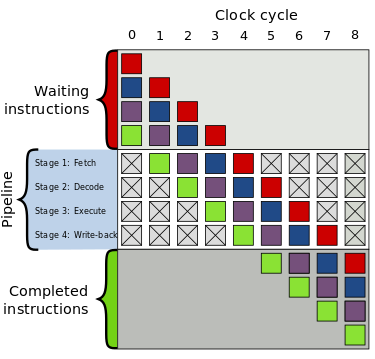
\includegraphics[width=0.4\textwidth]{pipeline}
	\caption{Schemat przykładowego procesora potowego}
	\label{pic:pip}
\end{figure}

Każda instrukcja składa się z czterech mikroinstrukcji. Kolorami (zielony, fioletowy, granatowy, czerwony) są zaznaczone kolejne instrukcje tego procesora, z których każda składa się z czterech mikroinstrukcji. Kolejne kolumny, to cykle procesora. Jak widać, od czwartego cyklu procesor kończy przetwarzanie jednej instrukcji w każdym cyklu, mimo że jedna instrukcja potrzebuje czterech cykli.

}
{W przetwarzaniu potokowym może być wykonywanych kilka instrukcji na raz, lecz te przetwarzanie każdej z tych instrukcji jest na różnych etapach.}

\answer{Sumator jednobitowy}{pozwala uzyskac sumę dwóch liczb jednobitowych z uwzględnieniem przeniesienia z poprzedniej pozycji}{T}
{
Układ kombinacyjny \ref{odp:90}. Implementacja [\ref{pic:sum}]
\begin{figure}
	\centering
	
\includegraphics[width=0.4\textwidth]{sumator}
	\caption{Sumator jednobitowy}
	\label{pic:sum}
\end{figure}

Sumatory wykonane tak jak na rysunku \ref{pic:sum}, można składać ze sobą tworząc sumator n-bitowy.
Dla i-tego sumatora jednobitowego w n-bitowym sumatorze:
\begin{itemize}
	\item wejście $A$, to i-ty bit pierwszego argumentu
	\item wejście $B$, to i-ty bit drugiego argumentu
	\item wejście $C_{in}$ jest podłączone do $C_{out}$ poprzedniego sumatora
	\item wyjście $S$, to i-ty bit sumy
	\item $C_{out}$, to i-ty bit przeniesienia.
\end{itemize}

}
{Służy po temu połączenie $C_{in}$ z $C_{out}$ poprzedniego sumatora}

\answer{Rejestr rozkazów}
{w trakcie wykonywania rozkazu zawartosć rejestru rozkazów musi zmienić się bezpośrednio przed pobraniem argumentu rozkazu z pamięci programu
}{T}
{
	Rejestr przechowujący obecnie przetwarzaną instrukcję. Którą instrukcję trzeba pobrać, określa licznik rozkazów \ref{odp:100}. Rejestr ten jest elementem jednostki sterującej \ref{odp:87} i wykorzystywany przez dekoder rozkazów.
}
{Rozkaz może określać sposób pobierania wartości. Argument nie musi być pobierany z pamięci, może być użyta wartość zachowana w rejestrach. Zastanawiające jest jednak słówko ,,bezpośrednio''.}

\answer{Przykłady układów kombinacyjnych, to}
{żaden z powyższych}{F}
{
	\begin{itemize}
		\item ALU
		\item sumator
		\item komparator
		\item (de)multiplexer
	\end{itemize}
	
}{nie żaden i tyle}

\answer{Przykłady układów sekwencyjnych, to}
{żaden z powyższych}{F}
{
Wszelkiego rodzaju przerzutniki i układy, w których skład one wchodzą (liczniki, rejestry itp.)
	
}{nie żaden i tyle}

\answer{Transmisja asynchroniczna}
{żaden z powyższych}{T}
{
	sposób przesyłania danych pozwalający na nieregularne ich wysyłanie, przy czym początek i koniec transmisji oznaczane są wydzielonym (ustalonym) symbolem.
	
}
{}

\begin{thebibliography}{99}
\bibitem{uw} Marcin Peczarski, \emph{Notatki do wykładu z architektury komputerów}, 17 lutego 2008
\bibitem{js} Notatki do kolosa \url{http://kolos.math.uni.lodz.pl/~archive/Architektura%20komputerow/07%20jednostka%20sterujaca.pdf}
\bibitem{uk} Układ kombinacyjny \url{https://pl.wikipedia.org/wiki/Uk%C5%82ad_kombinacyjny}
\bibitem{sram} Pamięć statyczna RAM \url{http://eduinf.waw.pl/inf/alg/002_struct/0043.php}
\bibitem{dram} Dynamiczna pamięć RAM \url{http://eduinf.waw.pl/inf/alg/002_struct/0044.php}
\bibitem{dwuport} Pamięć dwuportowa \url{https://pl.wikipedia.org/wiki/Pami%C4%99%C4%87_dwuportowa}
\bibitem{licz} Licznik asynchroniczny \url{http://eduinf.waw.pl/inf/alg/002_struct/0035.php}
\bibitem{fpga:hiw} How does an FPGA work? \url{https://embeddedmicro.com/tutorials/mojo-fpga-beginners-guide/how-does-an-fpga-work}
\bibitem{fpga:logi3D} Logi3D \url{http://www.logicbricks.com/Documentation/Flyers/logi3D_Graphics_Accelerator_01.pdf}
\end{thebibliography}

\setcounter{chapter}{12}
\chapter{Programowanie miktrokontrolerów i mikroprocesorów}
\PartialToc
%\startcontents[chapters]
%\printcontents[chapters]{}{1}{\section*{\contentsname}}
\setcounter{section}{215}

%-----------------
\answer
{Ile rejestrów 8-bitowych dostępnych dla programisty znajduje się w procesorach z rodziny x86?}
{6}
{F}
{8}
{
	Innej poprawnej nie ma. Rysunek poniżej
	\begin{center}
		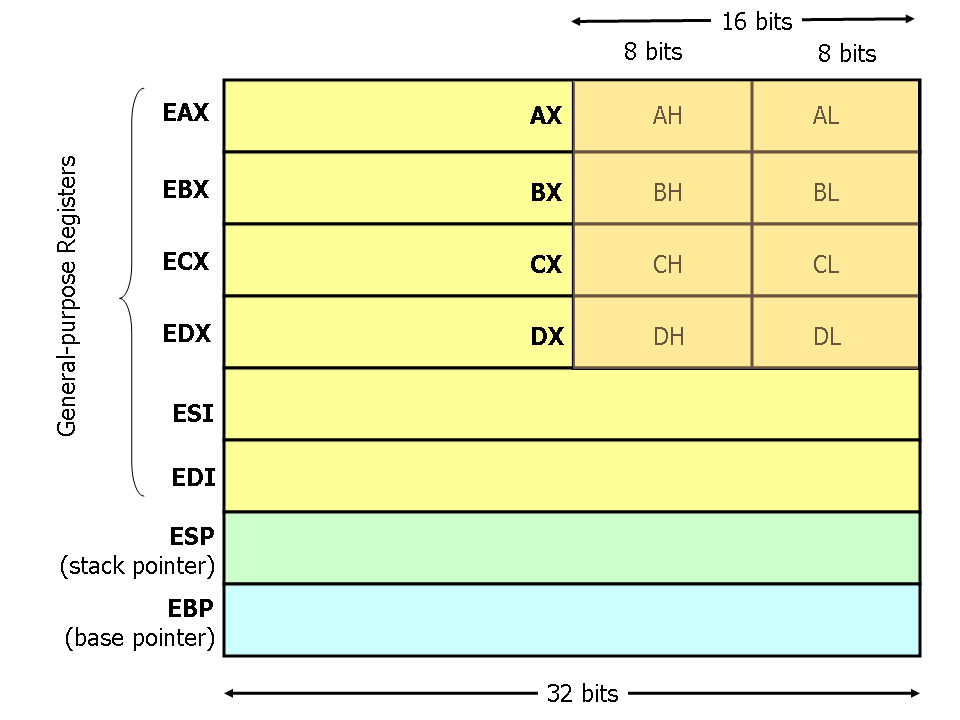
\includegraphics[width=6cm]{13/img/x86-registers.png}
		\captionof{figure}{Struktura rejestrów procka x86}
	\end{center}
}
%-----------------
\answer
{Jaki tryb adresowania wykorzystuje rozkaz ADDL (\%ebx),\%eax?\\}
{bezposredni}
{F}
{pośredni}
{
	Główny podział:
	\begin{itemize}
		\item bezpośredni (ang. direct)
		\item pośredni (ang. indirect)
	\end{itemize}
	Bardziej szczegółowo:
	\begin{itemize}
		\item rejestrowy (ang. register)
		\item rejestrowy pośredni (ang. register indirect)
		\item z przesunieciem (indeksowanie) (ang. displacement (indexed))
		\item stosowy (ang. stack)
	\end{itemize}
}
\begin{lstlisting}
bezposredni
movl 0x01, %eax
posredni
movl (%ebx), %eax
movl (%esi,%edi,1), %eax

\end{lstlisting}
%-----------------
\answer
{Jaka instrukcja jest równowazna w działaniu do instrukcji SHL \$1,\%eax?}
{SAL \$1,\%eax}
{T}
{}
{\\\textbf{SAL} - przesunięcie arytmetyczne w lewo\\
	\textbf{SHL} - przesunięcie bitowe w lewo.\\
	Przesuwanie w lewo czyli w stronę flagi CF. Przy ostatnim przesunięciu flaga zostanie wyzerowana więc nie ma znaczenia dla wyniku czy stosujemy arytmetyczne czy bitowe przesuniecie.}
\begin{lstlisting}
MOVW $0xFF00, %ax   #=> 0xff00 65280   # 1 1111 1111 0000 0000
SHL   $1, %eax      #=> 0x1fe00 130560 # 1 1111 1110 0000 0000
##
MOVW $0xFF00, %ax   #=> 0xff00 65280   # 1 1111 1111 0000 0000
SAL   $1, %eax      #=> 0x1fe00 130560 # 1 1111 1110 0000 0000

\end{lstlisting}
%-----------------%-----------------
\answer
{Która z ponizszych instrukcji dotyczy operacji na blokach danych?}
{STC}
{F}
{np. \textbf{MOV, PUSH, POP, XCHG, XLAT}}
{\begin{itemize}
		\item[] \textbf{STC} (STC/CLC - set carry / clear carry. Do flagi CF wstaw 1 lub 0, odpowiednio). \\FLAGI: \textbf{CF, OF, SF, ZF, IF, PF, DF} służą przede wszystkim do sterownia znacznikami np. do badania wyniku ostatniego przekształcenia (przepełnienie / wynik 0).
	\end{itemize}}
	%More - wykłądy Bublińskiego, Język asembler dla każdego Bogdan Drozdowski
	%-----------------%-----------------
	\answer
	{Według jakiej reguły moze być dokonywana konwersja do liczby całkowitej w jednostce FPU (Floating Point Unit)?
	}
	{round down}
	{T}
	{\\
		00 - round to nearest\\
		01 - round down\\
		10 - round up\\
		11 - round toward zero\\}
	{Powyżej możliwe ustawienia kontroli zaokrągleń w FPU. \\Źródło wykłady FTP wykłd 9. s16}
	%-----------------%-----------------
	\answer
	{Ile razy wykona sie pętla zbudowana w oparciu o instrukcję LOOP, jesli przed jej rozpoczeciem zawartosc rejestru \%ecx była równa 0? }
	{$2^{32}$}
	{T}
	{Chyba poprawne?}
	{rozkaz loop to petla for(\%ecx - -;\%ecx!=0;)\{\%ip+=disp\}. \\Źródło wykłady FTP}
	%-----------------%-----------------
	\answer
	{Ile razy zawartosc rejestru \%ah zostanie zapisana do pamieci poprzez uzycie instrukcji REP STOSB, jezeli przed jej wykonaniem zawartosc rejestru \%ecx była równa x?}
	{1}
	{F}
	{hmm czyżby chodzilo o zawartość al?, jeśli nie to zero razy bo STOSB wpisze AL nie AH, a jesli mial na mysli AL to x razy}
	{REP powtarza instrukcje x razy, w tym wypadku wezmie pod uwage rejestr CL jako licznik}
	%-----------------%-----------------
	\answer
	{
		Jaka bedzie zawartosc rejestru \%eax po sekwencji rozkazów?\\
		MOVL \$0xFFFF0000 ,\%eax\\
		NEG \%eax
	}
	{0x00000000}
	{F}
	{0x00010000}
	{
		\lstinputlisting{13/ideone_5Uwlpn.s}
	}
	%-----------------%-----------------
	\answer
	{Jaka bedzie zawartosc rejestru \%al po sekwencji rozkazów? \\
		MOVW \$0xFF00 ,\%ax\\
		ADCB \%ah ,\%al\\
		ADCB \%ah ,\%al\\
	}
	{nieokreslona}
	{F}
	{0xFFFE}
	{
		\lstinputlisting{13/ideone_13223.s}
	}
	%-----------------%-----------------
	\answer
	{Na jakim rodzaju schematu pokazane sa połaczenia elektryczne w układzie opartym na mikrokontrolerze?}
	{ideowym}
	{T}
	{?}
	{Schemat ideowy przedstawia w formie graficznej, jak mają zostać połączone poszczególne elementy.}
	%-----------------%-----------------
	\answer
	{W jakim rodzaju pamieci mikrokontrolera uzytkownik zwykle zapisuje kod programu?}
	{DRAM}
	{F}
	{
		\begin{itemize}
			\item EEPROM, Flash - zwykle
			\item EPROM, MRAM lub FRAM
		\end{itemize}
	}
	\\{Powyżej wymienione pamięci są pamięciami nieulotnymi, i tam umieszczamy kod programu.\\DRAM i SRAM są pamięciami ulotnymi, czyli po wyłączeniu zasilania kod przepada.}
	%-----------------%-----------------
	\answer
	{Jakie elementy wystepujace w mikrokontrolerach nie wystepuja w mikroprocesorach?}
	{ADC}
	{T}
	{}
	{\begin{itemize}
			\item Mikroprocesor to tylko:\\- \textbf{ALU} (Arithmetic Logic Unit) - jednostka licząca\\ - \textbf{CU} (Control Unit) - układ sterujący pracą\\ - \textbf{Rejestry}: PC, IR, SP - potrzebne przy wykonywaniu operacji obliczeniowych\\
			\item Mikrokontroler to układ w pełni autonomiczny, potrzebujący tylko zasilanie do pracy. Posiada w sobie procesor oraz peryferia np.:\\- pamięć danych do przechowywania kodu programu i zmiennych,\\- porty wejścia-wyjscia np: \textbf{ADC} (Analog-to-digital converter), \textbf{DAC},\\- układy czasowo-licznikowe, \\- kontrolery przerwań,\\- kontrolery transmisji\textbf{ UART, SPI, I2C, USB, CAN, 1-Wire} etc.,\\- zegar czasu rzeczywistego \textbf{RTC},\\- watchdog.
		\end{itemize}}
		%-----------------%-----------------
		\answer
		{Czy jezyk maszynowy jest tozsamy z jezykiem asemblera? }
		{nie}
		{T}
		{}
		{Język ASM to tekstowe odpowiedniki wewnętrznych rozkazów procesora (tzw. mnemoniki), kod maszynowy to po prostu liczby}
		%-----------------%-----------------
		\answer
		{Jakie narzedzie słuzy do zamiany kodu napisanego w jezyku asemblera na kod maszynowy? }
		{assembler}
		{T}
		{}
		{}
		%-----------------%-----------------
		\answer
		{Które z narzedzi nie umozliwia stworzenia kodu na mikrokontroler z rodziny AVR?}
		{Microsoft Visual Studio
		}
		{F}
		{Wszystkie narzędzia które nie wspierają Make, czyli da się np. w Eclipse, dedykowane do AVR jest AVR Studio}
		{http://www.instructables.com/id/Use-Visual-Studio-2010-to-Compile-AVR-Hex-Files/}
		%-----------------%-----------------

\end{document}